\documentclass[1p]{elsarticle_modified}
%\bibliographystyle{elsarticle-num}

%\usepackage[colorlinks]{hyperref}
%\usepackage{abbrmath_seonhwa} %\Abb, \Ascr, \Acal ,\Abf, \Afrak
\usepackage{amsfonts}
\usepackage{amssymb}
\usepackage{amsmath}
\usepackage{amsthm}
\usepackage{scalefnt}
\usepackage{amsbsy}
\usepackage{kotex}
\usepackage{caption}
\usepackage{subfig}
\usepackage{color}
\usepackage{graphicx}
\usepackage{xcolor} %% white, black, red, green, blue, cyan, magenta, yellow
\usepackage{float}
\usepackage{setspace}
\usepackage{hyperref}

\usepackage{tikz}
\usetikzlibrary{arrows}

\usepackage{multirow}
\usepackage{array} % fixed length table
\usepackage{hhline}

%%%%%%%%%%%%%%%%%%%%%
\makeatletter
\renewcommand*\env@matrix[1][\arraystretch]{%
	\edef\arraystretch{#1}%
	\hskip -\arraycolsep
	\let\@ifnextchar\new@ifnextchar
	\array{*\c@MaxMatrixCols c}}
\makeatother %https://tex.stackexchange.com/questions/14071/how-can-i-increase-the-line-spacing-in-a-matrix
%%%%%%%%%%%%%%%

\usepackage[normalem]{ulem}

\newcommand{\msout}[1]{\ifmmode\text{\sout{\ensuremath{#1}}}\else\sout{#1}\fi}
%SOURCE: \msout is \stkout macro in https://tex.stackexchange.com/questions/20609/strikeout-in-math-mode

\newcommand{\cancel}[1]{
	\ifmmode
	{\color{red}\msout{#1}}
	\else
	{\color{red}\sout{#1}}
	\fi
}

\newcommand{\add}[1]{
	{\color{blue}\uwave{#1}}
}

\newcommand{\replace}[2]{
	\ifmmode
	{\color{red}\msout{#1}}{\color{blue}\uwave{#2}}
	\else
	{\color{red}\sout{#1}}{\color{blue}\uwave{#2}}
	\fi
}

\newcommand{\Sol}{\mathcal{S}} %segment
\newcommand{\D}{D} %diagram
\newcommand{\A}{\mathcal{A}} %arc


%%%%%%%%%%%%%%%%%%%%%%%%%%%%%5 test

\def\sl{\operatorname{\textup{SL}}(2,\Cbb)}
\def\psl{\operatorname{\textup{PSL}}(2,\Cbb)}
\def\quan{\mkern 1mu \triangleright \mkern 1mu}

\theoremstyle{definition}
\newtheorem{thm}{Theorem}[section]
\newtheorem{prop}[thm]{Proposition}
\newtheorem{lem}[thm]{Lemma}
\newtheorem{ques}[thm]{Question}
\newtheorem{cor}[thm]{Corollary}
\newtheorem{defn}[thm]{Definition}
\newtheorem{exam}[thm]{Example}
\newtheorem{rmk}[thm]{Remark}
\newtheorem{alg}[thm]{Algorithm}

\newcommand{\I}{\sqrt{-1}}
\begin{document}

%\begin{frontmatter}
%
%\title{Boundary parabolic representations of knots up to 8 crossings}
%
%%% Group authors per affiliation:
%\author{Yunhi Cho} 
%\address{Department of Mathematics, University of Seoul, Seoul, Korea}
%\ead{yhcho@uos.ac.kr}
%
%
%\author{Seonhwa Kim} %\fnref{s_kim}}
%\address{Center for Geometry and Physics, Institute for Basic Science, Pohang, 37673, Korea}
%\ead{ryeona17@ibs.re.kr}
%
%\author{Hyuk Kim}
%\address{Department of Mathematical Sciences, Seoul National University, Seoul 08826, Korea}
%\ead{hyukkim@snu.ac.kr}
%
%\author{Seokbeom Yoon}
%\address{Department of Mathematical Sciences, Seoul National University, Seoul, 08826,  Korea}
%\ead{sbyoon15@snu.ac.kr}
%
%\begin{abstract}
%We find all boundary parabolic representation of knots up to 8 crossings.
%
%\end{abstract}
%\begin{keyword}
%    \MSC[2010] 57M25 
%\end{keyword}
%
%\end{frontmatter}

%\linenumbers
%\tableofcontents
%
\newcommand\colored[1]{\textcolor{white}{\rule[-0.35ex]{0.8em}{1.4ex}}\kern-0.8em\color{red} #1}%
%\newcommand\colored[1]{\textcolor{white}{ #1}\kern-2.17ex	\textcolor{white}{ #1}\kern-1.81ex	\textcolor{white}{ #1}\kern-2.15ex\color{red}#1	}

{\Large $\underline{11a_{91}~(K11a_{91})}$}

\setlength{\tabcolsep}{10pt}
\renewcommand{\arraystretch}{1.6}
\vspace{1cm}\begin{tabular}{m{100pt}>{\centering\arraybackslash}m{274pt}}
\multirow{5}{120pt}{
	\centering
	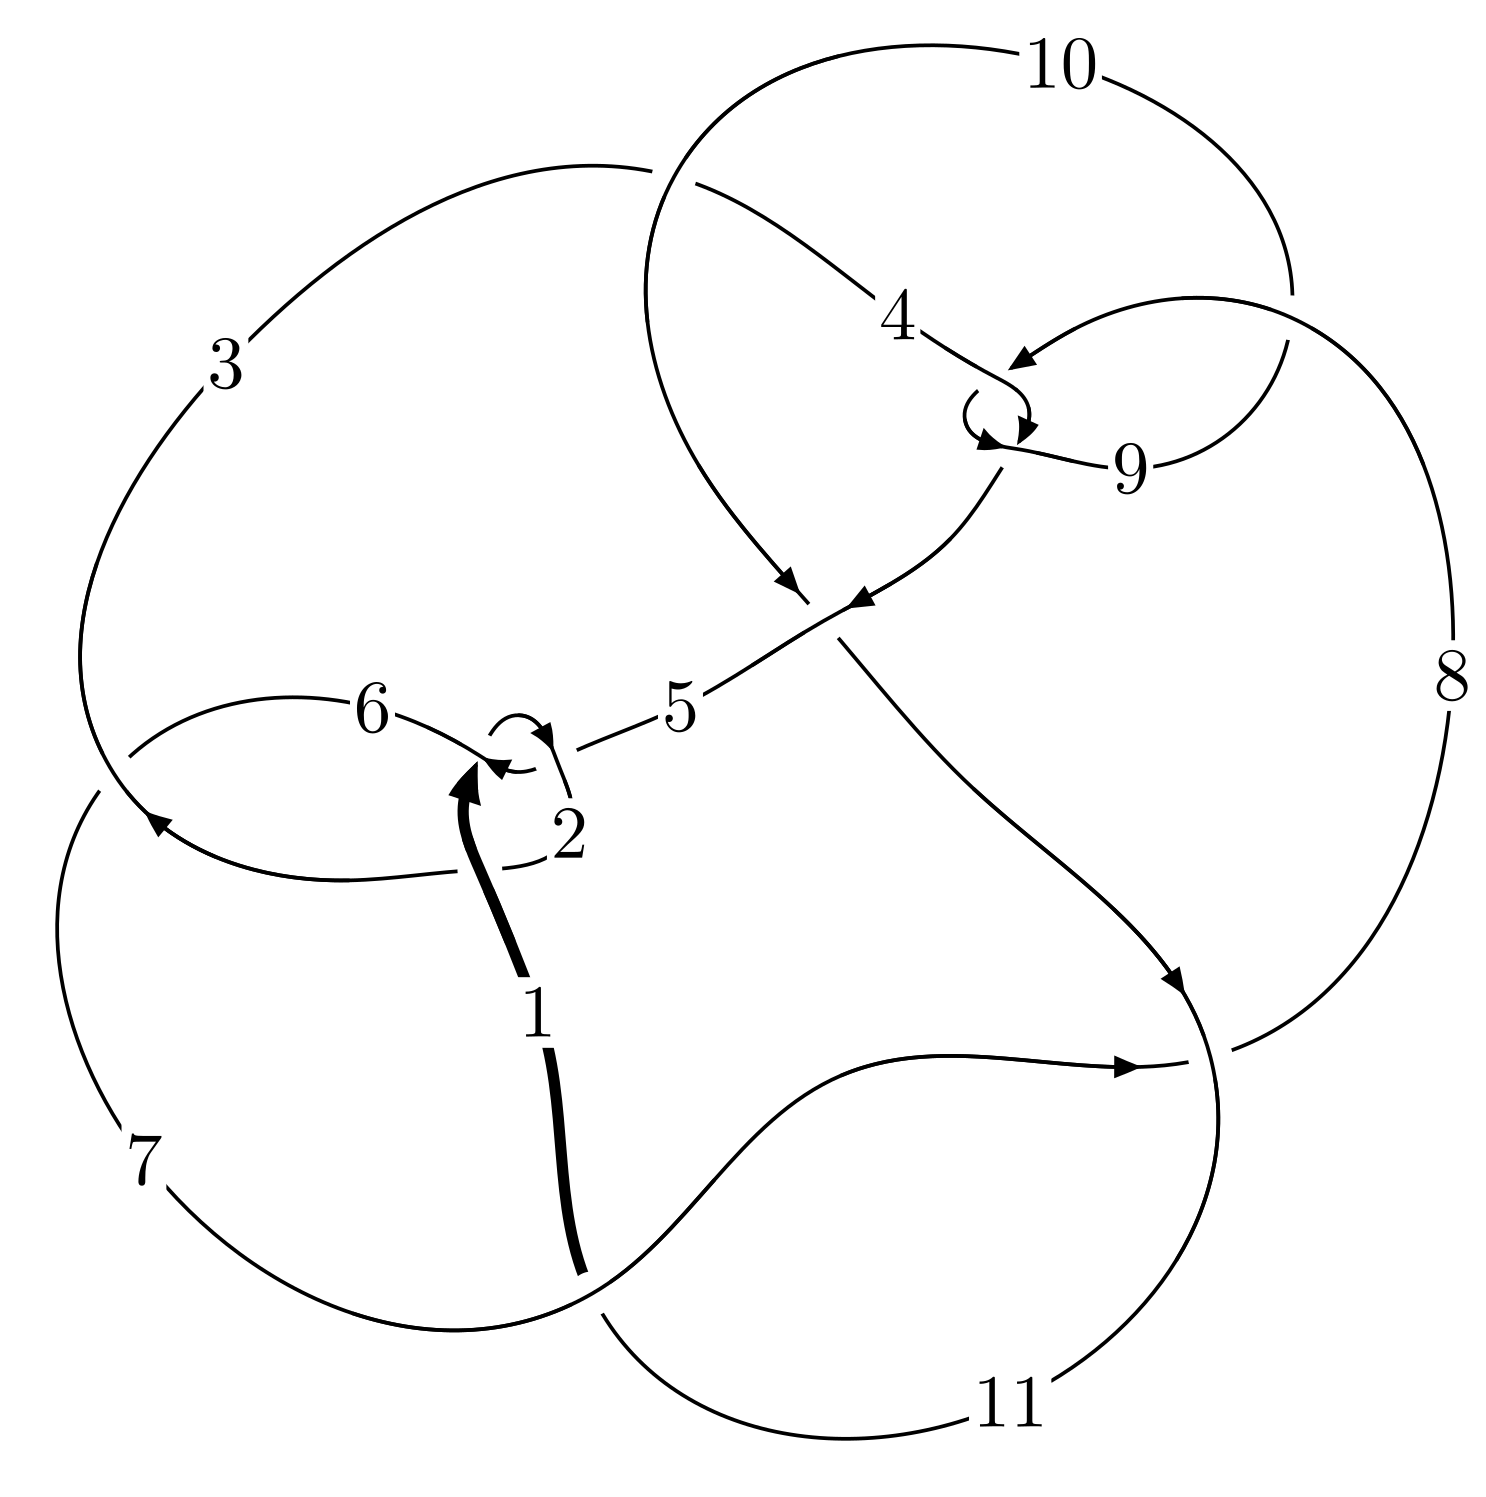
\includegraphics[width=112pt]{../../../GIT/diagram.site/Diagrams/png/340_11a_91.png}\\
\ \ \ A knot diagram\footnotemark}&
\allowdisplaybreaks
\textbf{Linearized knot diagam} \\
\cline{2-2}
 &
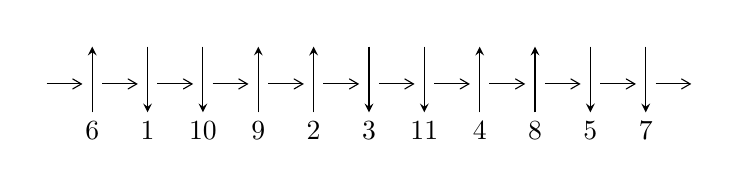
\begin{tikzpicture}[x=20pt, y=17pt]
	% nodes
	\node (C0) at (0, 0) {};
	\node (C1) at (1, 0) {};
	\node (C1U) at (1, +1) {};
	\node (C1D) at (1, -1) {6};

	\node (C2) at (2, 0) {};
	\node (C2U) at (2, +1) {};
	\node (C2D) at (2, -1) {1};

	\node (C3) at (3, 0) {};
	\node (C3U) at (3, +1) {};
	\node (C3D) at (3, -1) {10};

	\node (C4) at (4, 0) {};
	\node (C4U) at (4, +1) {};
	\node (C4D) at (4, -1) {9};

	\node (C5) at (5, 0) {};
	\node (C5U) at (5, +1) {};
	\node (C5D) at (5, -1) {2};

	\node (C6) at (6, 0) {};
	\node (C6U) at (6, +1) {};
	\node (C6D) at (6, -1) {3};

	\node (C7) at (7, 0) {};
	\node (C7U) at (7, +1) {};
	\node (C7D) at (7, -1) {11};

	\node (C8) at (8, 0) {};
	\node (C8U) at (8, +1) {};
	\node (C8D) at (8, -1) {4};

	\node (C9) at (9, 0) {};
	\node (C9U) at (9, +1) {};
	\node (C9D) at (9, -1) {8};

	\node (C10) at (10, 0) {};
	\node (C10U) at (10, +1) {};
	\node (C10D) at (10, -1) {5};

	\node (C11) at (11, 0) {};
	\node (C11U) at (11, +1) {};
	\node (C11D) at (11, -1) {7};
	\node (C12) at (12, 0) {};

	% arrows
	\draw[->,>={angle 60}]
	(C0) edge (C1) (C1) edge (C2) (C2) edge (C3) (C3) edge (C4) (C4) edge (C5) (C5) edge (C6) (C6) edge (C7) (C7) edge (C8) (C8) edge (C9) (C9) edge (C10) (C10) edge (C11) (C11) edge (C12) ;	\draw[->,>=stealth]
	(C1D) edge (C1U) (C2U) edge (C2D) (C3U) edge (C3D) (C4D) edge (C4U) (C5D) edge (C5U) (C6U) edge (C6D) (C7U) edge (C7D) (C8D) edge (C8U) (C9D) edge (C9U) (C10U) edge (C10D) (C11U) edge (C11D) ;
	\end{tikzpicture} \\
\hhline{~~} \\& 
\textbf{Solving Sequence} \\ \cline{2-2} 
 &
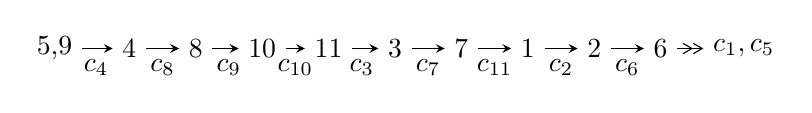
\begin{tikzpicture}[x=24pt, y=7pt]
	% node
	\node (A0) at (-1/8, 0) {5,9};
	\node (A1) at (1, 0) {4};
	\node (A2) at (2, 0) {8};
	\node (A3) at (3, 0) {10};
	\node (A4) at (4, 0) {11};
	\node (A5) at (5, 0) {3};
	\node (A6) at (6, 0) {7};
	\node (A7) at (7, 0) {1};
	\node (A8) at (8, 0) {2};
	\node (A9) at (9, 0) {6};
	\node (C1) at (1/2, -1) {$c_{4}$};
	\node (C2) at (3/2, -1) {$c_{8}$};
	\node (C3) at (5/2, -1) {$c_{9}$};
	\node (C4) at (7/2, -1) {$c_{10}$};
	\node (C5) at (9/2, -1) {$c_{3}$};
	\node (C6) at (11/2, -1) {$c_{7}$};
	\node (C7) at (13/2, -1) {$c_{11}$};
	\node (C8) at (15/2, -1) {$c_{2}$};
	\node (C9) at (17/2, -1) {$c_{6}$};
	\node (A10) at (41/4, 0) {$c_{1},c_{5}$};

	% edge
	\draw[->,>=stealth]	
	(A0) edge (A1) (A1) edge (A2) (A2) edge (A3) (A3) edge (A4) (A4) edge (A5) (A5) edge (A6) (A6) edge (A7) (A7) edge (A8) (A8) edge (A9) ;
	\draw[->>,>={angle 60}]	
	(A9) edge (A10);
\end{tikzpicture} \\ 

\end{tabular} \\

\footnotetext{
The image of knot diagram is generated by the software ``\textbf{Draw programme}" developed by Andrew Bartholomew(\url{http://www.layer8.co.uk/maths/draw/index.htm\#Running-draw}), where we modified some parts for our purpose(\url{https://github.com/CATsTAILs/LinksPainter}).
}\phantom \\ \newline 
\centering \textbf{Ideals for irreducible components\footnotemark of $X_{\text{par}}$} 
 
\begin{align*}
I^u_{1}&=\langle 
u^{64}- u^{63}+\cdots-2 u+1\rangle \\
\\
\end{align*}
\raggedright * 1 irreducible components of $\dim_{\mathbb{C}}=0$, with total 64 representations.\\
\footnotetext{All coefficients of polynomials are rational numbers. But the coefficients are sometimes approximated in decimal forms when there is not enough margin.}
\newpage
\renewcommand{\arraystretch}{1}
\centering \section*{I. $I^u_{1}= \langle u^{64}- u^{63}+\cdots-2 u+1 \rangle$}
\flushleft \textbf{(i) Arc colorings}\\
\begin{tabular}{m{7pt} m{180pt} m{7pt} m{180pt} }
\flushright $a_{5}=$&$\begin{pmatrix}1\\0\end{pmatrix}$ \\
\flushright $a_{9}=$&$\begin{pmatrix}0\\u\end{pmatrix}$ \\
\flushright $a_{4}=$&$\begin{pmatrix}1\\u^2\end{pmatrix}$ \\
\flushright $a_{8}=$&$\begin{pmatrix}- u\\- u^3+u\end{pmatrix}$ \\
\flushright $a_{10}=$&$\begin{pmatrix}u^3\\u^5- u^3+u\end{pmatrix}$ \\
\flushright $a_{11}=$&$\begin{pmatrix}- u^5+2 u^3- u\\u^5- u^3+u\end{pmatrix}$ \\
\flushright $a_{3}=$&$\begin{pmatrix}u^6- u^4+1\\u^8-2 u^6+2 u^4\end{pmatrix}$ \\
\flushright $a_{7}=$&$\begin{pmatrix}- u^{13}+4 u^{11}-7 u^9+6 u^7-2 u^5- u\\u^{13}-3 u^{11}+5 u^9-4 u^7+2 u^5- u^3+u\end{pmatrix}$ \\
\flushright $a_{1}=$&$\begin{pmatrix}- u^{21}+6 u^{19}+\cdots+2 u^3- u\\u^{21}-5 u^{19}+13 u^{17}-20 u^{15}+20 u^{13}-13 u^{11}+7 u^9-4 u^7+3 u^5- u^3+u\end{pmatrix}$ \\
\flushright $a_{2}=$&$\begin{pmatrix}u^{50}-13 u^{48}+\cdots+u^2+1\\- u^{50}+12 u^{48}+\cdots+4 u^4- u^2\end{pmatrix}$ \\
\flushright $a_{6}=$&$\begin{pmatrix}u^{27}-6 u^{25}+\cdots+4 u^7- u^3\\u^{29}-7 u^{27}+\cdots- u^3+u\end{pmatrix}$\\ \flushright $a_{6}=$&$\begin{pmatrix}u^{27}-6 u^{25}+\cdots+4 u^7- u^3\\u^{29}-7 u^{27}+\cdots- u^3+u\end{pmatrix}$\\&\end{tabular}
\flushleft \textbf{(ii) Obstruction class $= -1$}\\~\\
\flushleft \textbf{(iii) Cusp Shapes $= -4 u^{62}+60 u^{60}+\cdots+4 u-6$}\\~\\
\newpage\renewcommand{\arraystretch}{1}
\flushleft \textbf{(iv) u-Polynomials at the component}\newline \\
\begin{tabular}{m{50pt}|m{274pt}}
Crossings & \hspace{64pt}u-Polynomials at each crossing \\
\hline $$\begin{aligned}c_{1},c_{5}\end{aligned}$$&$\begin{aligned}
&u^{64}- u^{63}+\cdots-2 u+1
\end{aligned}$\\
\hline $$\begin{aligned}c_{2}\end{aligned}$$&$\begin{aligned}
&u^{64}+29 u^{63}+\cdots-16 u^4+1
\end{aligned}$\\
\hline $$\begin{aligned}c_{3}\end{aligned}$$&$\begin{aligned}
&u^{64}+3 u^{63}+\cdots+467 u+88
\end{aligned}$\\
\hline $$\begin{aligned}c_{4},c_{8}\end{aligned}$$&$\begin{aligned}
&u^{64}+u^{63}+\cdots+2 u+1
\end{aligned}$\\
\hline $$\begin{aligned}c_{6}\end{aligned}$$&$\begin{aligned}
&u^{64}+u^{63}+\cdots+11 u+2
\end{aligned}$\\
\hline $$\begin{aligned}c_{7},c_{11}\end{aligned}$$&$\begin{aligned}
&u^{64}-5 u^{63}+\cdots-32 u+1
\end{aligned}$\\
\hline $$\begin{aligned}c_{9}\end{aligned}$$&$\begin{aligned}
&u^{64}-31 u^{63}+\cdots+16 u^4+1
\end{aligned}$\\
\hline $$\begin{aligned}c_{10}\end{aligned}$$&$\begin{aligned}
&u^{64}- u^{63}+\cdots-8 u+1
\end{aligned}$\\
\hline
\end{tabular}\\~\\
\newpage\renewcommand{\arraystretch}{1}
\flushleft \textbf{(v) Riley Polynomials at the component}\newline \\
\begin{tabular}{m{50pt}|m{274pt}}
Crossings & \hspace{64pt}Riley Polynomials at each crossing \\
\hline $$\begin{aligned}c_{1},c_{5}\end{aligned}$$&$\begin{aligned}
&y^{64}+29 y^{63}+\cdots-16 y^4+1
\end{aligned}$\\
\hline $$\begin{aligned}c_{2}\end{aligned}$$&$\begin{aligned}
&y^{64}+13 y^{63}+\cdots-32 y^2+1
\end{aligned}$\\
\hline $$\begin{aligned}c_{3}\end{aligned}$$&$\begin{aligned}
&y^{64}+21 y^{63}+\cdots+151687 y+7744
\end{aligned}$\\
\hline $$\begin{aligned}c_{4},c_{8}\end{aligned}$$&$\begin{aligned}
&y^{64}-31 y^{63}+\cdots+16 y^4+1
\end{aligned}$\\
\hline $$\begin{aligned}c_{6}\end{aligned}$$&$\begin{aligned}
&y^{64}-3 y^{63}+\cdots-213 y+4
\end{aligned}$\\
\hline $$\begin{aligned}c_{7},c_{11}\end{aligned}$$&$\begin{aligned}
&y^{64}+49 y^{63}+\cdots-160 y+1
\end{aligned}$\\
\hline $$\begin{aligned}c_{9}\end{aligned}$$&$\begin{aligned}
&y^{64}+5 y^{63}+\cdots+32 y^2+1
\end{aligned}$\\
\hline $$\begin{aligned}c_{10}\end{aligned}$$&$\begin{aligned}
&y^{64}+y^{63}+\cdots+32 y+1
\end{aligned}$\\
\hline
\end{tabular}\\~\\
\newpage\flushleft \textbf{(vi) Complex Volumes and Cusp Shapes}
$$\begin{array}{c|c|c}  
\text{Solutions to }I^u_{1}& \I (\text{vol} + \sqrt{-1}CS) & \text{Cusp shape}\\
 \hline 
\begin{aligned}
u &= -0.939104 + 0.339205 I\end{aligned}
 & \phantom{-}1.65512 - 0.97415 I & \phantom{-}3.52790 + 1.04712 I \\ \hline\begin{aligned}
u &= -0.939104 - 0.339205 I\end{aligned}
 & \phantom{-}1.65512 + 0.97415 I & \phantom{-}3.52790 - 1.04712 I \\ \hline\begin{aligned}
u &= \phantom{-}0.844956 + 0.545528 I\end{aligned}
 & \phantom{-}0.03472 - 3.65450 I & -2.09839 + 2.07040 I \\ \hline\begin{aligned}
u &= \phantom{-}0.844956 - 0.545528 I\end{aligned}
 & \phantom{-}0.03472 + 3.65450 I & -2.09839 - 2.07040 I \\ \hline\begin{aligned}
u &= -0.784786 + 0.520323 I\end{aligned}
 & \phantom{-}1.84271 - 1.15146 I & \phantom{-}1.38817 + 3.13013 I \\ \hline\begin{aligned}
u &= -0.784786 - 0.520323 I\end{aligned}
 & \phantom{-}1.84271 + 1.15146 I & \phantom{-}1.38817 - 3.13013 I \\ \hline\begin{aligned}
u &= \phantom{-}0.925067 + 0.156259 I\end{aligned}
 & -0.18490 - 3.01523 I & \phantom{-}0.51085 + 4.08868 I \\ \hline\begin{aligned}
u &= \phantom{-}0.925067 - 0.156259 I\end{aligned}
 & -0.18490 + 3.01523 I & \phantom{-}0.51085 - 4.08868 I \\ \hline\begin{aligned}
u &= \phantom{-}0.691782 + 0.617995 I\end{aligned}
 & -0.43420 + 8.26774 I & -3.18319 - 8.31495 I \\ \hline\begin{aligned}
u &= \phantom{-}0.691782 - 0.617995 I\end{aligned}
 & -0.43420 - 8.26774 I & -3.18319 + 8.31495 I \\ \hline\begin{aligned}
u &= \phantom{-}0.948812 + 0.510706 I\end{aligned}
 & -1.98631 + 3.10078 I & -5.45245 - 3.88979 I \\ \hline\begin{aligned}
u &= \phantom{-}0.948812 - 0.510706 I\end{aligned}
 & -1.98631 - 3.10078 I & -5.45245 + 3.88979 I \\ \hline\begin{aligned}
u &= -0.701071 + 0.591063 I\end{aligned}
 & \phantom{-}1.52804 - 3.28439 I & \phantom{-}0.17422 + 4.06730 I \\ \hline\begin{aligned}
u &= -0.701071 - 0.591063 I\end{aligned}
 & \phantom{-}1.52804 + 3.28439 I & \phantom{-}0.17422 - 4.06730 I \\ \hline\begin{aligned}
u &= \phantom{-}0.622278 + 0.585266 I\end{aligned}
 & -2.93619 + 1.29722 I & -7.30833 - 2.92067 I \\ \hline\begin{aligned}
u &= \phantom{-}0.622278 - 0.585266 I\end{aligned}
 & -2.93619 - 1.29722 I & -7.30833 + 2.92067 I \\ \hline\begin{aligned}
u &= -1.071540 + 0.414993 I\end{aligned}
 & \phantom{-}2.79512 - 1.45588 I & \phantom{-0.000000 } 0 \\ \hline\begin{aligned}
u &= -1.071540 - 0.414993 I\end{aligned}
 & \phantom{-}2.79512 + 1.45588 I & \phantom{-0.000000 } 0 \\ \hline\begin{aligned}
u &= -1.122750 + 0.278948 I\end{aligned}
 & \phantom{-}2.73183 + 0.05760 I & \phantom{-0.000000 } 0 \\ \hline\begin{aligned}
u &= -1.122750 - 0.278948 I\end{aligned}
 & \phantom{-}2.73183 - 0.05760 I & \phantom{-0.000000 } 0 \\ \hline\begin{aligned}
u &= -1.036170 + 0.550652 I\end{aligned}
 & -3.04852 - 2.03669 I & \phantom{-0.000000 } 0 \\ \hline\begin{aligned}
u &= -1.036170 - 0.550652 I\end{aligned}
 & -3.04852 + 2.03669 I & \phantom{-0.000000 } 0 \\ \hline\begin{aligned}
u &= \phantom{-}0.294713 + 0.772195 I\end{aligned}
 & \phantom{-}1.49417 - 10.13740 I & -1.81004 + 7.03416 I \\ \hline\begin{aligned}
u &= \phantom{-}0.294713 - 0.772195 I\end{aligned}
 & \phantom{-}1.49417 + 10.13740 I & -1.81004 - 7.03416 I \\ \hline\begin{aligned}
u &= \phantom{-}1.090790 + 0.461542 I\end{aligned}
 & \phantom{-}2.45432 + 5.70994 I & \phantom{-0.000000 } 0 \\ \hline\begin{aligned}
u &= \phantom{-}1.090790 - 0.461542 I\end{aligned}
 & \phantom{-}2.45432 - 5.70994 I & \phantom{-0.000000 } 0 \\ \hline\begin{aligned}
u &= -0.284380 + 0.763443 I\end{aligned}
 & \phantom{-}3.48322 + 4.95658 I & \phantom{-}1.27407 - 2.78403 I \\ \hline\begin{aligned}
u &= -0.284380 - 0.763443 I\end{aligned}
 & \phantom{-}3.48322 - 4.95658 I & \phantom{-}1.27407 + 2.78403 I \\ \hline\begin{aligned}
u &= -1.156900 + 0.262634 I\end{aligned}
 & \phantom{-}5.97549 + 7.09510 I & \phantom{-0.000000 } 0 \\ \hline\begin{aligned}
u &= -1.156900 - 0.262634 I\end{aligned}
 & \phantom{-}5.97549 - 7.09510 I & \phantom{-0.000000 } 0\\
 \hline 
 \end{array}$$\newpage$$\begin{array}{c|c|c}  
\text{Solutions to }I^u_{1}& \I (\text{vol} + \sqrt{-1}CS) & \text{Cusp shape}\\
 \hline 
\begin{aligned}
u &= \phantom{-}1.154850 + 0.273654 I\end{aligned}
 & \phantom{-}7.87867 - 1.87799 I & \phantom{-0.000000 } 0 \\ \hline\begin{aligned}
u &= \phantom{-}1.154850 - 0.273654 I\end{aligned}
 & \phantom{-}7.87867 + 1.87799 I & \phantom{-0.000000 } 0 \\ \hline\begin{aligned}
u &= -0.487387 + 0.645472 I\end{aligned}
 & -4.65712 - 2.64556 I & -8.69821 + 3.84156 I \\ \hline\begin{aligned}
u &= -0.487387 - 0.645472 I\end{aligned}
 & -4.65712 + 2.64556 I & -8.69821 - 3.84156 I \\ \hline\begin{aligned}
u &= \phantom{-}1.064500 + 0.535808 I\end{aligned}
 & \phantom{-}0.17913 + 5.31802 I & \phantom{-0.000000 } 0 \\ \hline\begin{aligned}
u &= \phantom{-}1.064500 - 0.535808 I\end{aligned}
 & \phantom{-}0.17913 - 5.31802 I & \phantom{-0.000000 } 0 \\ \hline\begin{aligned}
u &= \phantom{-}1.154460 + 0.302003 I\end{aligned}
 & \phantom{-}8.21168 + 1.00289 I & \phantom{-0.000000 } 0 \\ \hline\begin{aligned}
u &= \phantom{-}1.154460 - 0.302003 I\end{aligned}
 & \phantom{-}8.21168 - 1.00289 I & \phantom{-0.000000 } 0 \\ \hline\begin{aligned}
u &= -1.155880 + 0.315108 I\end{aligned}
 & \phantom{-}6.59460 - 6.19283 I & \phantom{-0.000000 } 0 \\ \hline\begin{aligned}
u &= -1.155880 - 0.315108 I\end{aligned}
 & \phantom{-}6.59460 + 6.19283 I & \phantom{-0.000000 } 0 \\ \hline\begin{aligned}
u &= -0.423078 + 0.678155 I\end{aligned}
 & -4.36286 + 4.56971 I & -7.67331 - 4.88314 I \\ \hline\begin{aligned}
u &= -0.423078 - 0.678155 I\end{aligned}
 & -4.36286 - 4.56971 I & -7.67331 + 4.88314 I \\ \hline\begin{aligned}
u &= \phantom{-}0.304810 + 0.731968 I\end{aligned}
 & -1.50287 - 2.92329 I & -5.31775 + 2.36689 I \\ \hline\begin{aligned}
u &= \phantom{-}0.304810 - 0.731968 I\end{aligned}
 & -1.50287 + 2.92329 I & -5.31775 - 2.36689 I \\ \hline\begin{aligned}
u &= -1.070330 + 0.558396 I\end{aligned}
 & -2.47375 - 9.35788 I & \phantom{-0.000000 } 0 \\ \hline\begin{aligned}
u &= -1.070330 - 0.558396 I\end{aligned}
 & -2.47375 + 9.35788 I & \phantom{-0.000000 } 0 \\ \hline\begin{aligned}
u &= -0.248813 + 0.743811 I\end{aligned}
 & \phantom{-}4.02540 + 2.21650 I & \phantom{-}2.22128 - 2.47627 I \\ \hline\begin{aligned}
u &= -0.248813 - 0.743811 I\end{aligned}
 & \phantom{-}4.02540 - 2.21650 I & \phantom{-}2.22128 + 2.47627 I \\ \hline\begin{aligned}
u &= \phantom{-}0.226658 + 0.736100 I\end{aligned}
 & \phantom{-}2.50217 + 2.88719 I & -0.11514 - 2.73367 I \\ \hline\begin{aligned}
u &= \phantom{-}0.226658 - 0.736100 I\end{aligned}
 & \phantom{-}2.50217 - 2.88719 I & -0.11514 + 2.73367 I \\ \hline\begin{aligned}
u &= \phantom{-}0.421396 + 0.617038 I\end{aligned}
 & -1.69065 - 0.75291 I & -4.16901 + 1.04385 I \\ \hline\begin{aligned}
u &= \phantom{-}0.421396 - 0.617038 I\end{aligned}
 & -1.69065 + 0.75291 I & -4.16901 - 1.04385 I \\ \hline\begin{aligned}
u &= \phantom{-}1.126510 + 0.550942 I\end{aligned}
 & \phantom{-}0.88876 + 7.79459 I & \phantom{-0.000000 } 0 \\ \hline\begin{aligned}
u &= \phantom{-}1.126510 - 0.550942 I\end{aligned}
 & \phantom{-}0.88876 - 7.79459 I & \phantom{-0.000000 } 0 \\ \hline\begin{aligned}
u &= \phantom{-}1.142880 + 0.528499 I\end{aligned}
 & \phantom{-}5.14617 + 1.86555 I & \phantom{-0.000000 } 0 \\ \hline\begin{aligned}
u &= \phantom{-}1.142880 - 0.528499 I\end{aligned}
 & \phantom{-}5.14617 - 1.86555 I & \phantom{-0.000000 } 0 \\ \hline\begin{aligned}
u &= -1.141810 + 0.537319 I\end{aligned}
 & \phantom{-}6.61499 - 7.03708 I & \phantom{-0.000000 } 0 \\ \hline\begin{aligned}
u &= -1.141810 - 0.537319 I\end{aligned}
 & \phantom{-}6.61499 + 7.03708 I & \phantom{-0.000000 } 0 \\ \hline\begin{aligned}
u &= -1.140370 + 0.553325 I\end{aligned}
 & \phantom{-}5.98813 - 9.90485 I & \phantom{-0.000000 } 0 \\ \hline\begin{aligned}
u &= -1.140370 - 0.553325 I\end{aligned}
 & \phantom{-}5.98813 + 9.90485 I & \phantom{-0.000000 } 0\\
 \hline 
 \end{array}$$\newpage$$\begin{array}{c|c|c}  
\text{Solutions to }I^u_{1}& \I (\text{vol} + \sqrt{-1}CS) & \text{Cusp shape}\\
 \hline 
\begin{aligned}
u &= \phantom{-}1.140530 + 0.558856 I\end{aligned}
 & \phantom{-}3.9773 + 15.1327 I & \phantom{-0.000000 } 0 \\ \hline\begin{aligned}
u &= \phantom{-}1.140530 - 0.558856 I\end{aligned}
 & \phantom{-}3.9773 - 15.1327 I & \phantom{-0.000000 } 0 \\ \hline\begin{aligned}
u &= \phantom{-}0.109376 + 0.527151 I\end{aligned}
 & -0.08646 - 1.82443 I & -0.12496 + 3.83658 I \\ \hline\begin{aligned}
u &= \phantom{-}0.109376 - 0.527151 I\end{aligned}
 & -0.08646 + 1.82443 I & -0.12496 - 3.83658 I\\
 \hline 
 \end{array}$$\newpage
\newpage\renewcommand{\arraystretch}{1}
\centering \section*{ II. u-Polynomials}
\begin{tabular}{m{50pt}|m{274pt}}
Crossings & \hspace{64pt}u-Polynomials at each crossing \\
\hline $$\begin{aligned}c_{1},c_{5}\end{aligned}$$&$\begin{aligned}
&u^{64}- u^{63}+\cdots-2 u+1
\end{aligned}$\\
\hline $$\begin{aligned}c_{2}\end{aligned}$$&$\begin{aligned}
&u^{64}+29 u^{63}+\cdots-16 u^4+1
\end{aligned}$\\
\hline $$\begin{aligned}c_{3}\end{aligned}$$&$\begin{aligned}
&u^{64}+3 u^{63}+\cdots+467 u+88
\end{aligned}$\\
\hline $$\begin{aligned}c_{4},c_{8}\end{aligned}$$&$\begin{aligned}
&u^{64}+u^{63}+\cdots+2 u+1
\end{aligned}$\\
\hline $$\begin{aligned}c_{6}\end{aligned}$$&$\begin{aligned}
&u^{64}+u^{63}+\cdots+11 u+2
\end{aligned}$\\
\hline $$\begin{aligned}c_{7},c_{11}\end{aligned}$$&$\begin{aligned}
&u^{64}-5 u^{63}+\cdots-32 u+1
\end{aligned}$\\
\hline $$\begin{aligned}c_{9}\end{aligned}$$&$\begin{aligned}
&u^{64}-31 u^{63}+\cdots+16 u^4+1
\end{aligned}$\\
\hline $$\begin{aligned}c_{10}\end{aligned}$$&$\begin{aligned}
&u^{64}- u^{63}+\cdots-8 u+1
\end{aligned}$\\
\hline
\end{tabular}\newpage\renewcommand{\arraystretch}{1}
\centering \section*{ III. Riley Polynomials}
\begin{tabular}{m{50pt}|m{274pt}}
Crossings & \hspace{64pt}Riley Polynomials at each crossing \\
\hline $$\begin{aligned}c_{1},c_{5}\end{aligned}$$&$\begin{aligned}
&y^{64}+29 y^{63}+\cdots-16 y^4+1
\end{aligned}$\\
\hline $$\begin{aligned}c_{2}\end{aligned}$$&$\begin{aligned}
&y^{64}+13 y^{63}+\cdots-32 y^2+1
\end{aligned}$\\
\hline $$\begin{aligned}c_{3}\end{aligned}$$&$\begin{aligned}
&y^{64}+21 y^{63}+\cdots+151687 y+7744
\end{aligned}$\\
\hline $$\begin{aligned}c_{4},c_{8}\end{aligned}$$&$\begin{aligned}
&y^{64}-31 y^{63}+\cdots+16 y^4+1
\end{aligned}$\\
\hline $$\begin{aligned}c_{6}\end{aligned}$$&$\begin{aligned}
&y^{64}-3 y^{63}+\cdots-213 y+4
\end{aligned}$\\
\hline $$\begin{aligned}c_{7},c_{11}\end{aligned}$$&$\begin{aligned}
&y^{64}+49 y^{63}+\cdots-160 y+1
\end{aligned}$\\
\hline $$\begin{aligned}c_{9}\end{aligned}$$&$\begin{aligned}
&y^{64}+5 y^{63}+\cdots+32 y^2+1
\end{aligned}$\\
\hline $$\begin{aligned}c_{10}\end{aligned}$$&$\begin{aligned}
&y^{64}+y^{63}+\cdots+32 y+1
\end{aligned}$\\
\hline
\end{tabular}
\vskip 2pc
\end{document}